\documentclass[10pt,letterpaper]{article} 
\usepackage{tikz}
\usepackage{tools}
\usepackage{enumitem,caption}
\usepackage{listings}
\lstset{language=Python}
%\lstset{frame=lines}
%\lstset{caption={Insert code directly in your document}}
\lstset{label={lst:code_direct}}
\lstset{basicstyle=\footnotesize}

%\usepackage{graphicx}‎‎
%\usefonttheme{serif}‎
%\usepackage{ptext}‎
%\usepackage{xepersian}
%\settextfont{B Nazanin}
\usepackage{lipsum}
\setlength{\parindent}{0pt}
\newcommand{\pf}{$\blacksquare$}

\newcommand{\Span}{\text{Span}}
\newcommand{\NF}{\text{NF}}
\newcommand{\EDFA}{\text{EDFA}}
\newcommand{\ASE}{\text{ASE}}

\newcommand{\bns}{\textit{broadcast-and-select}  architecture}
\newcommand{\Bns}{\textit{Broadcast-and-select} architecture}

\newcommand{\rns}{\textit{route-and-select} architecture}
\newcommand{\Rns}{\textit{Route-and-select} architecture}

\newcounter{QuestionNumber}
\setcounter{QuestionNumber}{1}

\newcommand{\temp}{{\color{red}{temp}}}

\newcommand{\Q}{
\textbf{Question \theQuestionNumber)}
\stepcounter{QuestionNumber}
}
\newcommand{\EX}{\Bbb E}
\newcommand{\nl}{\newline\newline}
\begin{document}
\large
\begin{center}
In the name of beauty

The 8th problem set of Optical Networks course
\hl
\end{center}

\Q

\begin{enumerate}[label=\alph*-]
\item
Which one of multistep RWA and one-step RWA imposes more practical complexity? Which one of those algorithms yields better results usually? Suppose that a network is not heavily loaded. Which algorithm is better to be deployed and why?
\item
What is the motivation of using Most-Used algorithm in wavelength assignment?
\end{enumerate}

\Q

Given the following network topology,
\begin{figure}[h]
\centering
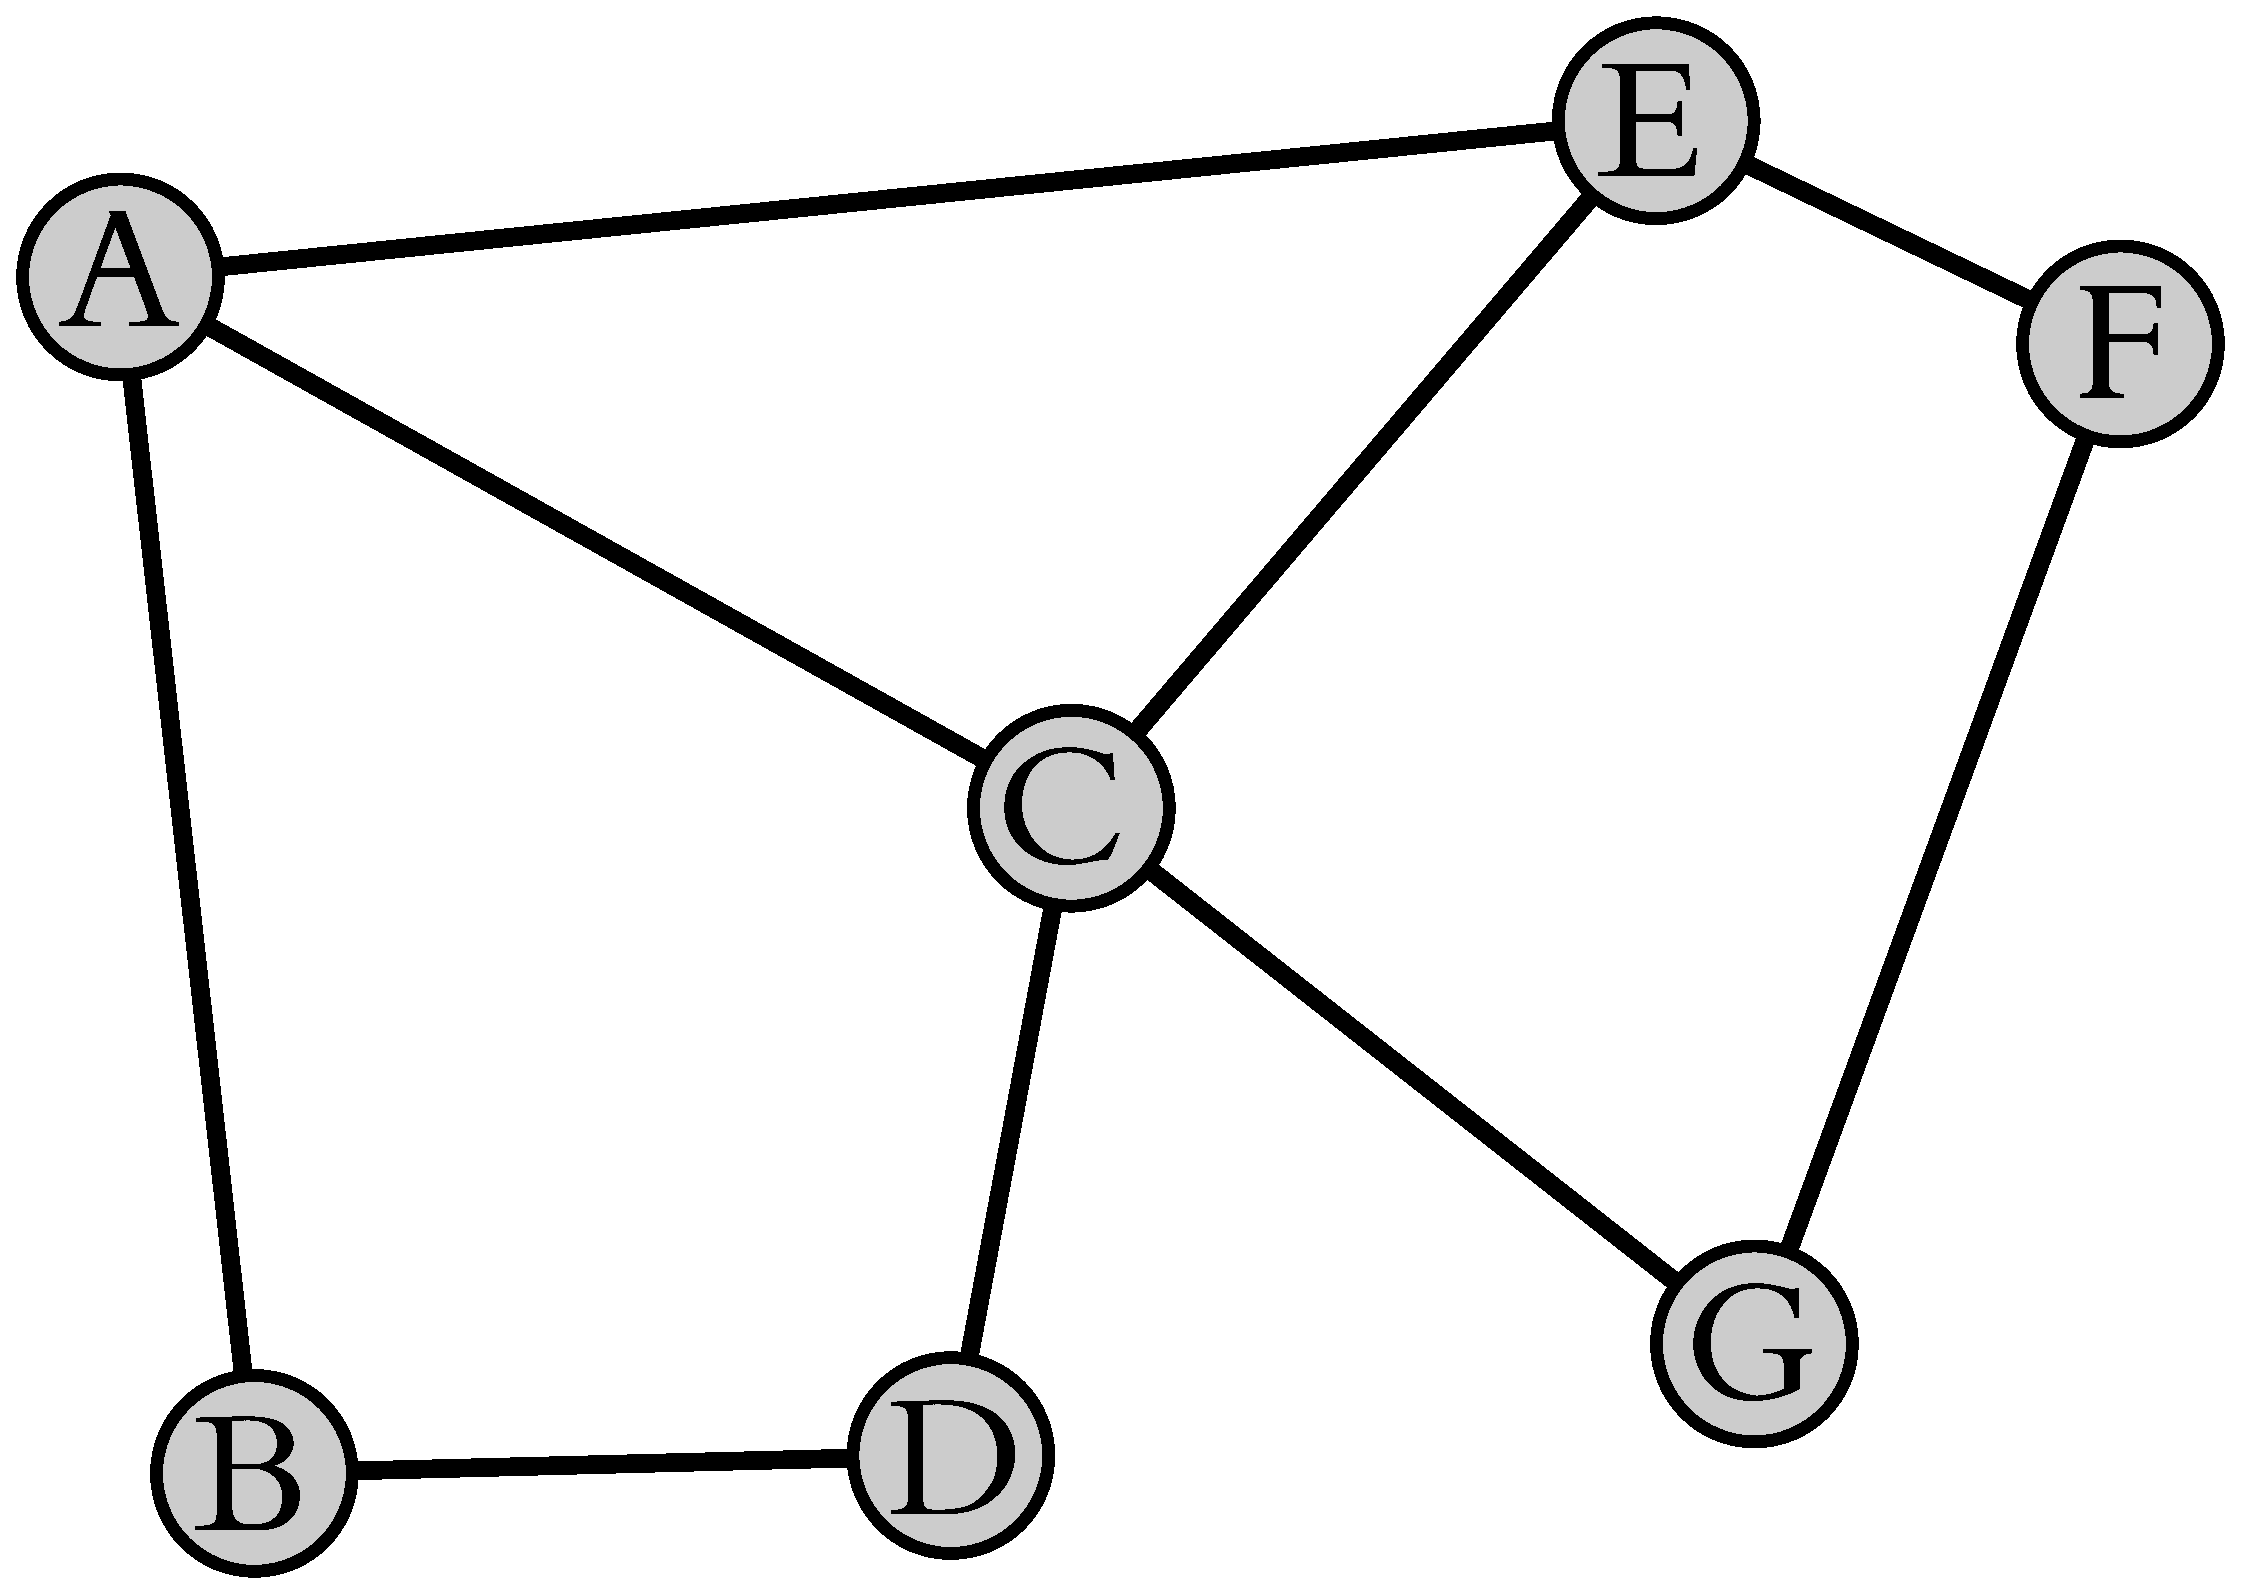
\includegraphics[width=60mm]{net-wa.eps}
\end{figure}

and the following set of lightpaths,
{
\begin{table}[h]
\Large
\centering
\begin{tabular}{|c|c|}
\hline
Lightpath ID&Nodelist\\
\hline
1&E-A-C\\
\hline
2&A-C-G-F\\
\hline
3&F-E-C-D\\
\hline
4&B-D-C\\
\hline
5&A-B-D\\
\hline
6&C-G\\
\hline
7&C-D-B\\
\hline
\end{tabular}
\end{table}
}

perform the wavelength assignment procedure using
\begin{enumerate}[label=\alph*-]
\item
first-fit
\item
most-used.
\end{enumerate}

\newpage

\Q

In the following network, the free wavelength indices on links are denoted by green-colored sets (link DB has no free wavelength at the time of RWA).
\begin{figure}[h]
\centering
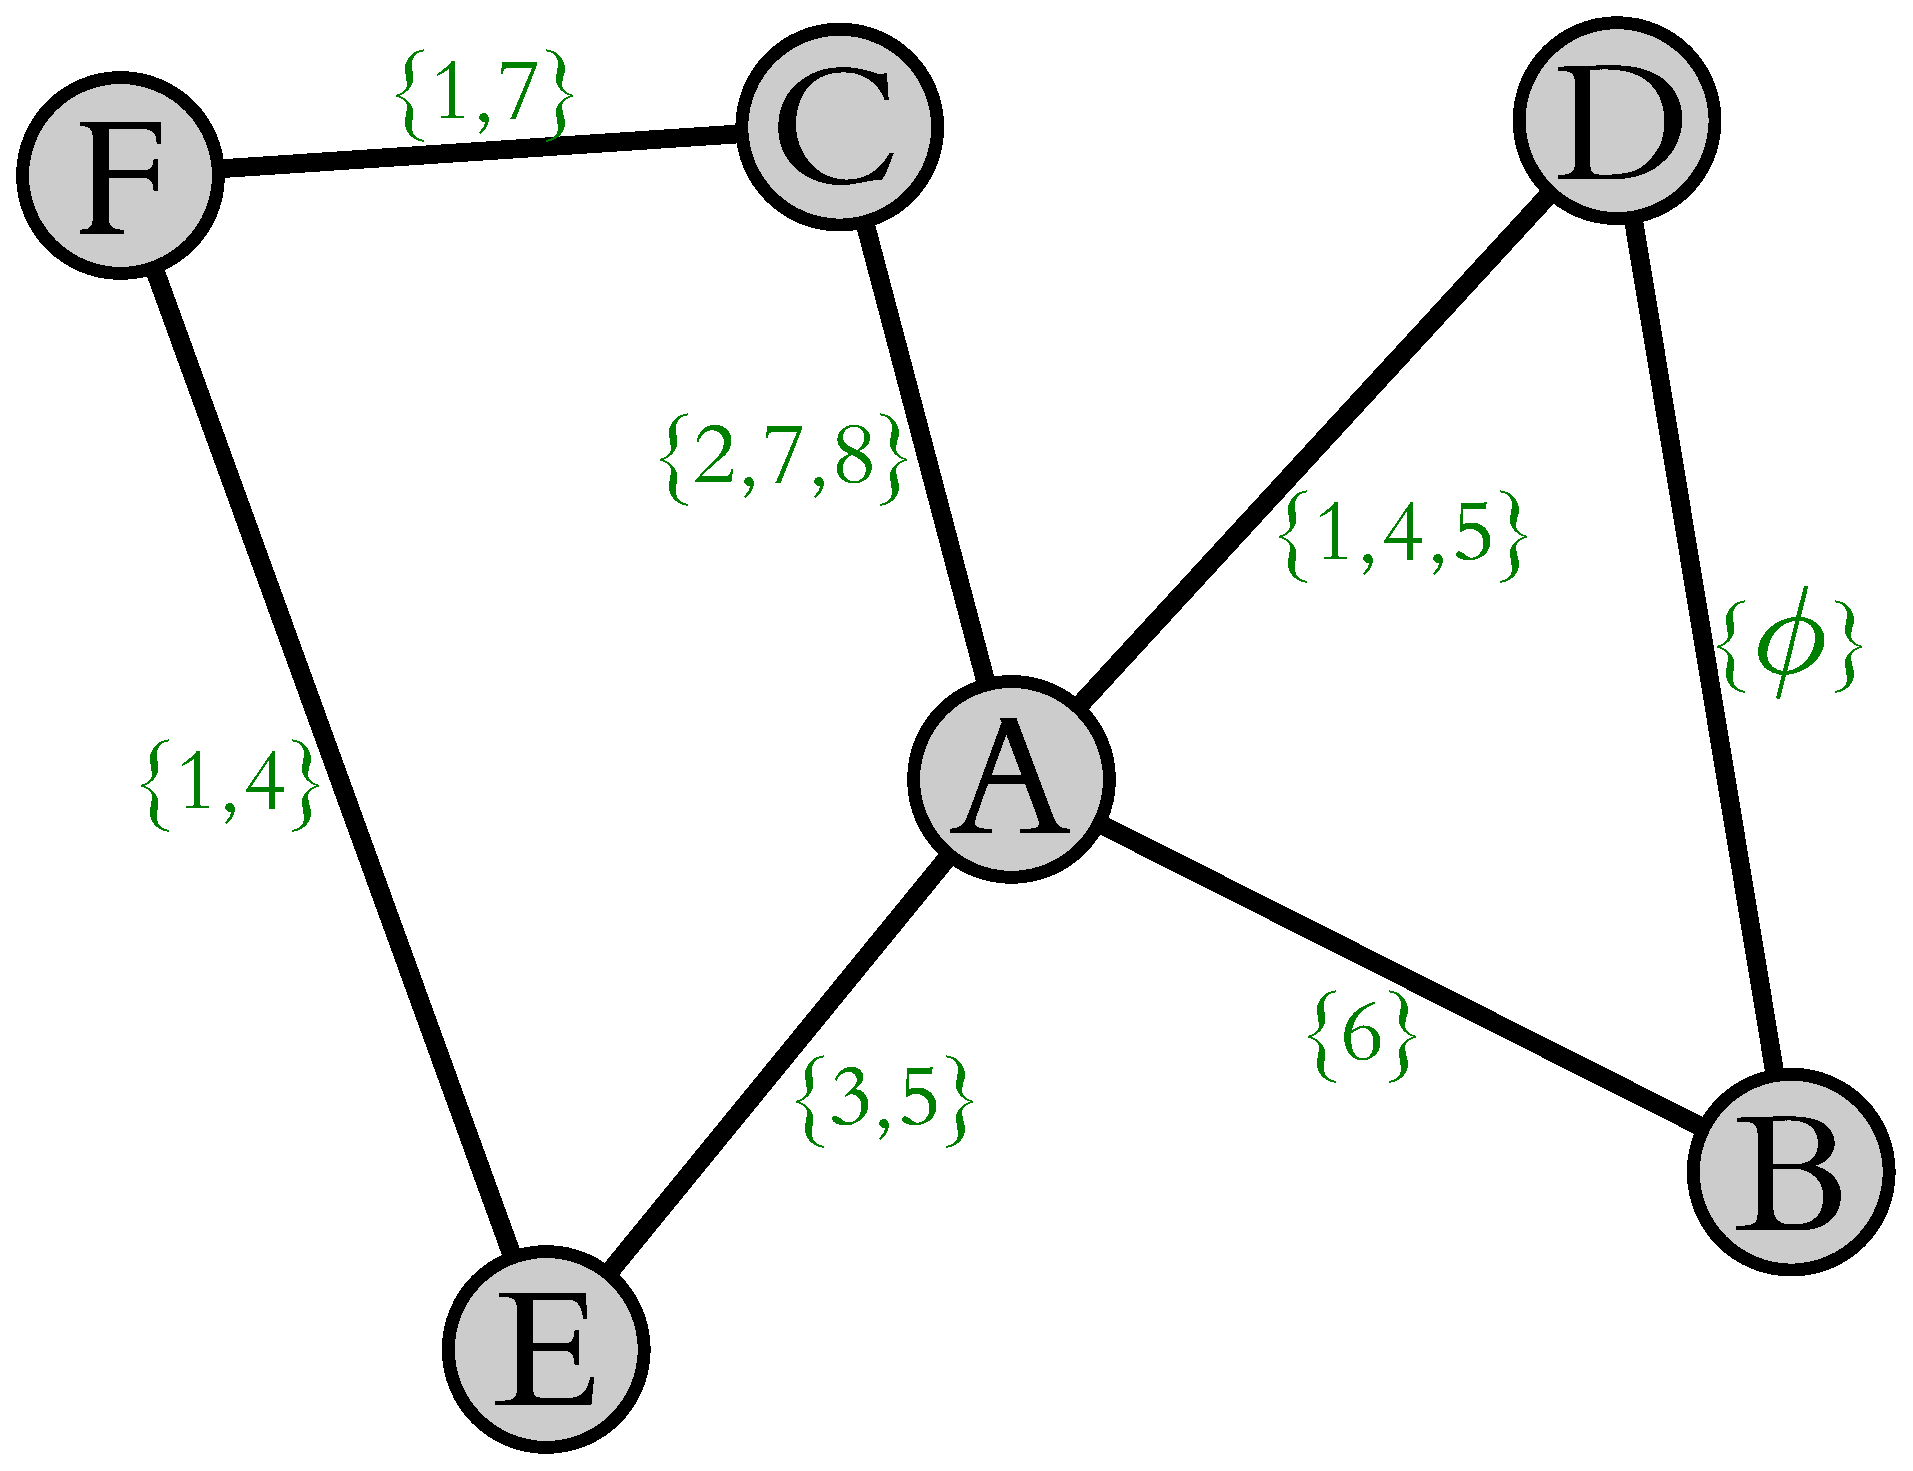
\includegraphics[width=60mm]{net-wa-tp.eps}
\end{figure}

\begin{enumerate}[label=\alph*-]
\item
Perform topology pruning to find a route and an allocated wavelength for each of the two demands between source-destination pairs E-D and F-B all optically. Is there any demand blocked?
\item
How can regeneration solve the problem of blocked services? Explain your solution.
\end{enumerate}

\end{document}